\chapter{La Formula di Green}

\section{Definizione e Orientazione}
La formula di Green stabilisce una relazione fondamentale tra l'integrale di linea (circuitazione) lungo una curva chiusa e l'integrale doppio esteso alla regione piana racchiusa da tale curva.

Sia $\vec{F}(x,y) = (F_1, F_2)$ un campo vettoriale e sia $\sigma$ un dominio del piano. La Formula di Green afferma che:
\[
\oint_{\partial \sigma} F_1 \, dx + F_2 \, dy = \iint_{\sigma} \left( \frac{\partial F_2}{\partial x} - \frac{\partial F_1}{\partial y} \right) dx \, dy
\]
dove $\partial \sigma$ è la frontiera orientata di $\sigma$. 

\subsection{Cosa vuol dire orientata in modo "opportuno"?}
Affinché il teorema sia valido, bisogna percorrere la curva $\partial \sigma$ \textbf{lasciando il dominio sempre sulla sinistra}. 
Questo significa che per un dominio semplice (senza buchi), la curva esterna deve essere percorsa in senso \textbf{antiorario}.

\begin{figure}[H]
    \centering
    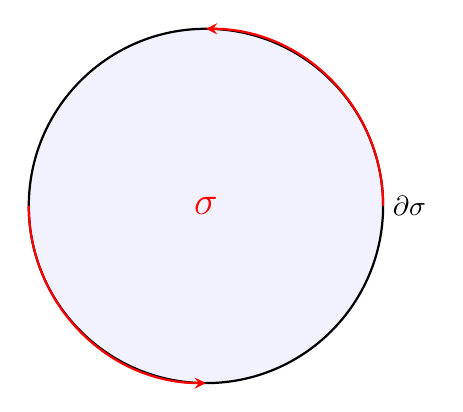
\begin{tikzpicture}[scale=1.5, >=stealth]
        % Dominio semplice
        \fill[blue!5] (0,0) circle (1.5);
        \draw[thick] (0,0) circle (1.5);
        
        % Frecce manuali per l'orientazione antioraria
        \draw[thick, red, ->] (1.5,0) arc (0:90:1.5);
        \draw[thick, red, ->] (-1.5,0) arc (180:270:1.5);
        
        \node[red, font=\Large] at (0,0) {$\sigma$};
        \node[right] at (1.5, 0) {$\partial \sigma$};
    \end{tikzpicture}
    \caption{Dominio semplice: la frontiera $\partial \sigma$ è orientata in senso antiorario.}
\end{figure}

\subsection{Domini con "buchi" (Multiconnessi)}
Se la regione ha dei buchi, la regola di "lasciare il dominio a sinistra" implica che:
\begin{itemize}
    \item La curva esterna è orientata in senso \textbf{antiorario}.
    \item Le curve interne (le frontiere dei buchi) sono orientate in senso \textbf{orario}.
\end{itemize}

\begin{figure}[H]
    \centering
    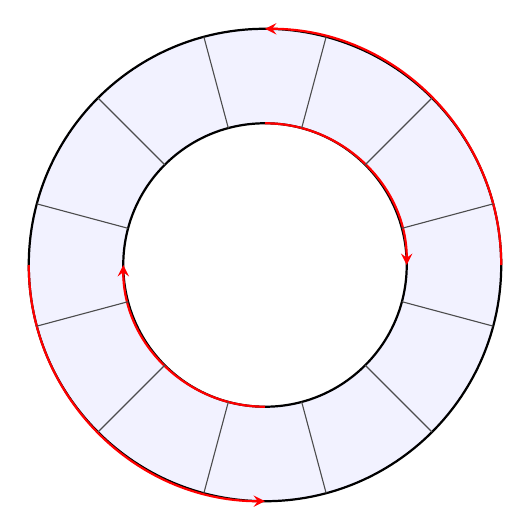
\begin{tikzpicture}[scale=1.5, >=stealth]
        % Dominio con buco (colorazione con even odd rule)
        \fill[blue!5, even odd rule] (0,0) circle (2) (0,0) circle (1.2);
        
        % Curva esterna 
        \draw[thick] (0,0) circle (2);
        % Frecce esterne (antiorarie)
        \draw[thick, red, ->] (2,0) arc (0:90:2);
        \draw[thick, red, ->] (-2,0) arc (180:270:2);
        
        % Curva interna
        \draw[thick] (0,0) circle (1.2);
        % Frecce interne (orarie)
        \draw[thick, red, <-] (1.2,0) arc (0:90:1.2);
        \draw[thick, red, <-] (-1.2,0) arc (180:270:1.2);
        
        % Tratteggio (simulando gli appunti a mano)
        \foreach \a in {15, 45, ..., 345} {
            \draw[thin, black!70] (\a:1.2) -- (\a:2);
        }
    \end{tikzpicture}
    \caption{Dominio multiconnesso: curva esterna antioraria, curva interna oraria.}
\end{figure}

\section{Domini Semplici}

Un dominio $\sigma$ si definisce \textbf{semplice} se è l'unione di un numero finito di regioni di tipo 1 (rispetto all'asse $x$) e simultaneamente l'unione di un numero finito di regioni di tipo 2 (rispetto all'asse $y$). Le regioni si intersecano al più lungo le loro frontiere.

\section{Dimostrazione della Formula di Green}
Devo dimostrare la correttezza della formula dividendo il problema in due identità:
\begin{align}
    \oint_{\partial \sigma} F_1 \, dx &= -\iint_{\sigma} \frac{\partial F_1}{\partial y} \, dx \, dy \label{eq:green1} \\
    \oint_{\partial \sigma} F_2 \, dy &= \iint_{\sigma} \frac{\partial F_2}{\partial x} \, dx \, dy \label{eq:green2}
\end{align}
Dimostro la prima identità \eqref{eq:green1}, visto che la seconda \eqref{eq:green2} si dimostra in modo del tutto analogo.

\begin{enumerate}
    \item \textbf{Scomposizione:} Uso l'ipotesi che $\sigma$ può essere diviso in un numero finito di regioni $\sigma_i$ di tipo 1.
    \item \textbf{Analisi della singola regione:} Consideriamo una generica sottoregione $\sigma_i$ di tipo 1.
    \item \textbf{Basta dimostrare l'identità per $\sigma_i$:} 
    \[
    \oint_{\partial \sigma_i} F_1 \, dx = -\iint_{\sigma_i} \frac{\partial F_1}{\partial y} \, dx \, dy
    \]
    dove $\partial \sigma_i$ è la frontiera orientata di $\sigma_i$.
    \item \textbf{Somma sui domini:} Se la relazione vale per ogni singola $\sigma_i$, allora sommando su tutti gli $N$ sottodomini si ha:
    \[
    \sum_{i=1}^{N} \oint_{\partial \sigma_i} F_1 \, dx = \oint_{\partial \sigma} F_1 \, dx = - \sum_{i=1}^{N} \iint_{\sigma_i} \frac{\partial F_1}{\partial y} \, dx \, dy = - \iint_{\sigma} \frac{\partial F_1}{\partial y} \, dx \, dy
    \]
    \textit{(Nota: gli integrali lungo i tratti di taglio interni si elidono a coppie perché percorsi in versi opposti).}
    
    \item \textbf{Calcolo dell'integrale di linea:} Consideriamo $\sigma_i$ definita da $a \le x \le b$ e $y_1(x) \le y \le y_2(x)$.
    Scomponendo l'integrale di linea sui 4 lati (inferiore, destro, superiore, sinistro), notiamo che sui segmenti verticali $dx = 0$, quindi non contribuiscono:
    \[
    \oint_{\partial \sigma_i} F_1(x,y) \, dx = \int_{a}^{b} F_1(x, y_1(x)) \, dx + \int_{b}^{a} F_1(x, y_2(x)) \, dx
    \]
    Invertendo gli estremi del secondo integrale otteniamo:
    \[
    \oint_{\partial \sigma_i} F_1 \, dx = \int_{a}^{b} \left[ F_1(x, y_1(x)) - F_1(x, y_2(x)) \right] dx
    \]

    \item \textbf{Calcolo dell'integrale doppio:} Dall'altra parte dell'uguaglianza, calcoliamo l'integrale doppio usando le formule di riduzione per domini di tipo 1:
    \begin{align*}
        -\iint_{\sigma_i} \frac{\partial F_1}{\partial y} \, dx \, dy &= - \int_{a}^{b} dx \int_{y_1(x)}^{y_2(x)} \frac{\partial F_1}{\partial y} \, dy \\
        &= - \int_{a}^{b} \left[ F_1(x, y) \right]_{y_1(x)}^{y_2(x)} dx \\
        &= - \int_{a}^{b} \left[ F_1(x, y_2(x)) - F_1(x, y_1(x)) \right] dx \\
        &= \int_{a}^{b} \left[ F_1(x, y_1(x)) - F_1(x, y_2(x)) \right] dx
    \end{align*}    
    I risultati del punto 5 e del punto 6 sono identici. L'identità è dimostrata.
\end{enumerate}

\section{Conseguenze della formula di Green e Lemma di Poincaré}
Dato un campo vettoriale $\vec{F} = F_1 \vec{e}_1 + \dots + F_n \vec{e}_n$, esso è conservativo (ovvero $\vec{F} = \vec{\nabla} U \iff F_i = \frac{\partial U}{\partial x_i}$) se rispetta le condizioni necessarie di irrotazionalità:
\begin{equation*}
    \frac{\partial F_i}{\partial x_j} = \frac{\partial F_j}{\partial x_i} \quad \text{con } i \neq j
\end{equation*}
Inoltre, se il dominio di definizione è \textbf{semplicemente connesso}, le condizioni necessarie sono anche \textbf{sufficienti}.

\subsection{Lemma di Poincaré (Dimostrazione tramite Green)}

Ipotizziamo che il dominio di definizione del campo piano $\vec{F} = F_1 \vec{e}_1 + F_2 \vec{e}_2$ sia semplicemente connesso.
Se il campo è irrotazionale, applicando la Formula di Green su una qualsiasi curva chiusa $C$ (che racchiude una superficie $\sigma$ interamente contenuta nel dominio), otteniamo:
\begin{equation*}
    \oint_C \vec{F} \cdot d\vec{r} = \iint_\sigma \left( \frac{\partial F_2}{\partial x} - \frac{\partial F_1}{\partial y} \right) d\sigma = 0
\end{equation*}
Poiché la circuitazione è nulla su ogni percorso chiuso, il campo è conservativo.

\subsection{Che effetti hanno le conseguenze di Green sul Lemma di Poincaré?}

La Formula di Green è letteralmente il ``motore matematico'' che fa funzionare il Lemma di Poincaré in due dimensioni. 

Il Lemma di Poincaré afferma che: \textbf{se un campo vettoriale è irrotazionale e il suo dominio è semplicemente connesso, allora è sicuramente conservativo}. Ma \emph{perché} l'irrotazionalità garantisce che sia conservativo? È qui che entra in gioco la Formula di Green. 

Essa crea un ponte tra il bordo di una regione e il suo interno, affermando che la circuitazione di un campo $\vec{F}$ lungo una curva chiusa $C$ è uguale all'integrale doppio della quantità $\left(\frac{\partial F_2}{\partial x} - \frac{\partial F_1}{\partial y}\right)$ sull'area $\sigma$ racchiusa dalla curva. 

Ecco l'effetto a catena:
\begin{itemize}
    \item \textbf{L'effetto dell'irrotazionalità:} Se il campo soddisfa le condizioni necessarie (è irrotazionale), sappiamo che $\frac{\partial F_2}{\partial x} = \frac{\partial F_1}{\partial y}$. Inserendo questa uguaglianza nel lato destro della Formula di Green, la funzione integranda diventa zero.
    \item \textbf{L'effetto della circuitazione nulla:} Poiché l'integrale doppio si annulla, anche la circuitazione (il lato sinistro di Green) deve fare zero ($\oint_C \vec{F} \cdot d\vec{r} = 0$). Se la circuitazione su una qualsiasi curva chiusa è nulla, significa che il lavoro non dipende dal cammino percorso. Questa è l'esatta definizione di \textbf{campo conservativo}.
\end{itemize}

\subsubsection{Perché il dominio \emph{deve} essere semplicemente connesso?}

Questo è il dettaglio topologico fondamentale che fa crollare o reggere il teorema. La Formula di Green funziona \textbf{solo se tutta l'area $\sigma$ racchiusa dalla curva $C$ fa interamente parte del dominio del campo}.

Se il dominio avesse un ``buco'' (ovvero non fosse semplicemente connesso) e la curva $C$ girasse intorno a quel buco, non sarebbe possibile calcolare l'integrale doppio di Green sull'area racchiusa, poiché in quel buco il campo non esiste o non è ben definito. Di conseguenza, il fatto che le derivate incrociate siano uguali non garantirebbe più l'annullamento della circuitazione. 
L'ipotesi che il dominio sia semplicemente connesso garantisce, invece, che ogni curva chiusa racchiuda \emph{esclusivamente} punti in cui il campo è valido e regolare.